\chapter{Introduction}
% If you don't want quotes, comment the next lines.
\begin{flushright}
Cool quote at the begining of first chapter...\\
\emph{- Someone awesome (Extract from...) -}
\end{flushright}
Some introduction on the topic to talk about. Maybe you're talking about nonlinear 
acoustics and directional speakers. Maybe talk on this chapter about the the concept,
be sure to define the problem and some of the pathway to solving it. Don't 
overcomplicate it. \medskip\\
This chapter should define the problems you want to address, the objectives, the 
scope, methodology and structure of the document.
\section{Definition of the problem} % Planteamiento del problema
El problema a resolver en este trabajo es modelar matemáticamente el comportamiento 
de una bocina direccional\footnote{everyone loves footnotes, so throw some in there!}
,...
\section{Objectives and Scope}
You must be able to determine a list of objectives you want to fulfill, and how far
does your research contemplate. Maybe something like:
\begin{itemize}
\item Build the math models, trying to make sense of them into your application. You 
want to understand further the phenomena you're studying, and math is a great tool.
\item Maybe some practical work might be in order, like a programing or an actual 
experiment
\item Throw in something exiting and new.
\end{itemize}
Since you can't cover absolutely everything, it is smart to talk about the scope of
your work. Where it fails, what won't it consider...
\section{Structure and methodology}
Methodology to solve the problem, and structure to explain what is going to be 
covered and where on the document. I sense another list coming...
\begin{figure}[hbpt]
\centering
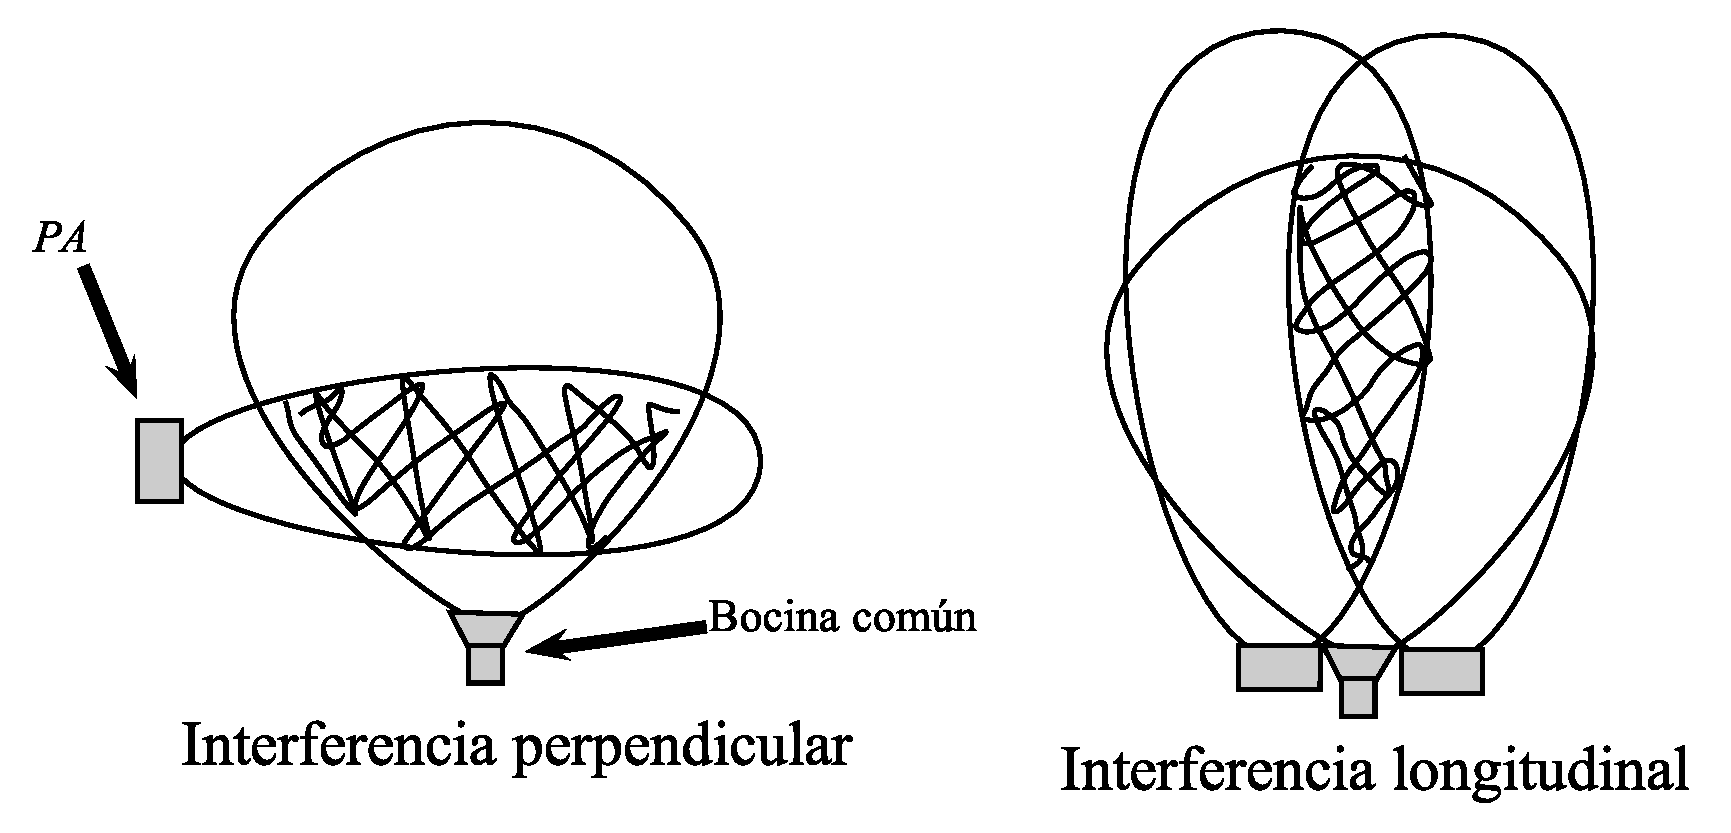
\includegraphics[scale=0.31]{introexp}
\caption{Caption for the image (Where did you get this?)}
\label{fig:introexp}
\end{figure}
Explain Figure \ref{fig:introexp} properly. 